\chapter{数的整除性}
\begin{introduction}[本章内容提要]
	\item 欧几里得算法
	\item 拓展欧几里得算法
\end{introduction}

\section{最小公倍数}
两个数a与b(不全为零)的最大公因数是整除它们两个的最大数,记为$gcd(a,b)$。如果$gcd(a,b)=1$,我们称$a$与$b$互质。

求两个数最大公因数的最有效的方法是{\heiti 欧几里得算法},其核心操作是辗转相除,先看一个例子。

\begin{example}
	欧几里得算法求gcd(28,93)的例子。
	
	第一步用93除以28得商为3,余数为7,记作下面式子:
	$$
		93 = 3*28 + 7
	$$
	第二步用上一步的除数作为新的被除数,上一步的余数作为新的除数,即:
	$$
		28 = 4*7 + 0
	$$
	发现此时余数为0,算法不再继续。欧几里得算法指出当得到余数0时,除数(上一步的余数)就是最初两个数的最大公因数。所以
	gcd(28,93) = 7。
\end{example}

\begin{theorem}{欧几里得算法}{label}
	要计算两个整数a与b的GCD,先令$r_{-1}=a$且$r_{0}=b$,然后计算相继的商和余数:$r_{i-1}=q_{i+1}*r_{i}+r_{i+1} \quad (i=0,1,2,...)$,
	直到某余数$r_{n+1}=0$,最后的非零余数$r_{n}$就是a与b的最大公因数。
\end{theorem}

\begin{proof}
	考虑一般情形,有
	\begin{align*}
	r_{-1} &= q_1*r_0 + r_1 \\
	r_0 &= q_2*r_1 + r_2 \\
	r_1 &= q_3 * r_2 + r_3 \\
	r_2 &= q_4 * r_3 + r_4 \\
 	&\cdot \cdot \cdot\\
	r_{n-3} &= q_{n-1}*r_{n-2} + r_{n-1} \\
	r_{n-2} &= q_{n} * r_{n-1} + {\color{red} r_n} \\
	r_{n-1} &= q_{n+1} * r_n + 0 \\
	\end{align*}
	欧几里得算法说,最后的$r_n$就是gcd,那么我们先证明$r_n$一定是$a(r_{-1})$和$b(r_0)$的因子。
	
	由最后一行知,$r_n$整除$r_{n-1}$,于是由倒数第二行知$r_n$整除$r_{n-2}$,依次类推,$r_n$整除$r_{0}$和$r_{-1}$。
	
	下面再证明$r_n$是$a$与$b$的{\heiti 最大}公因数。假设$d$是$a$与$b$的任意公因数,则由上面式子第一行知$d$整除$r_1$,
	于是由第二行知$d$整除$r_2$,依次类推,$d$整除$r_n$,即$r_n$是最大的公因数。
	
	最后,还要说明一定存在$r_{n+1}$为0,易知,每一次余数都是严格递减的,所以余数最后总能到0。那自然会问,要多少步呢?
	实际上,{\heiti 欧几里得算法的步数至多是$b$的位数的7倍}。
\end{proof}



\section{线性方程定理}
test




























\begin{figure}[htbp]
\centering
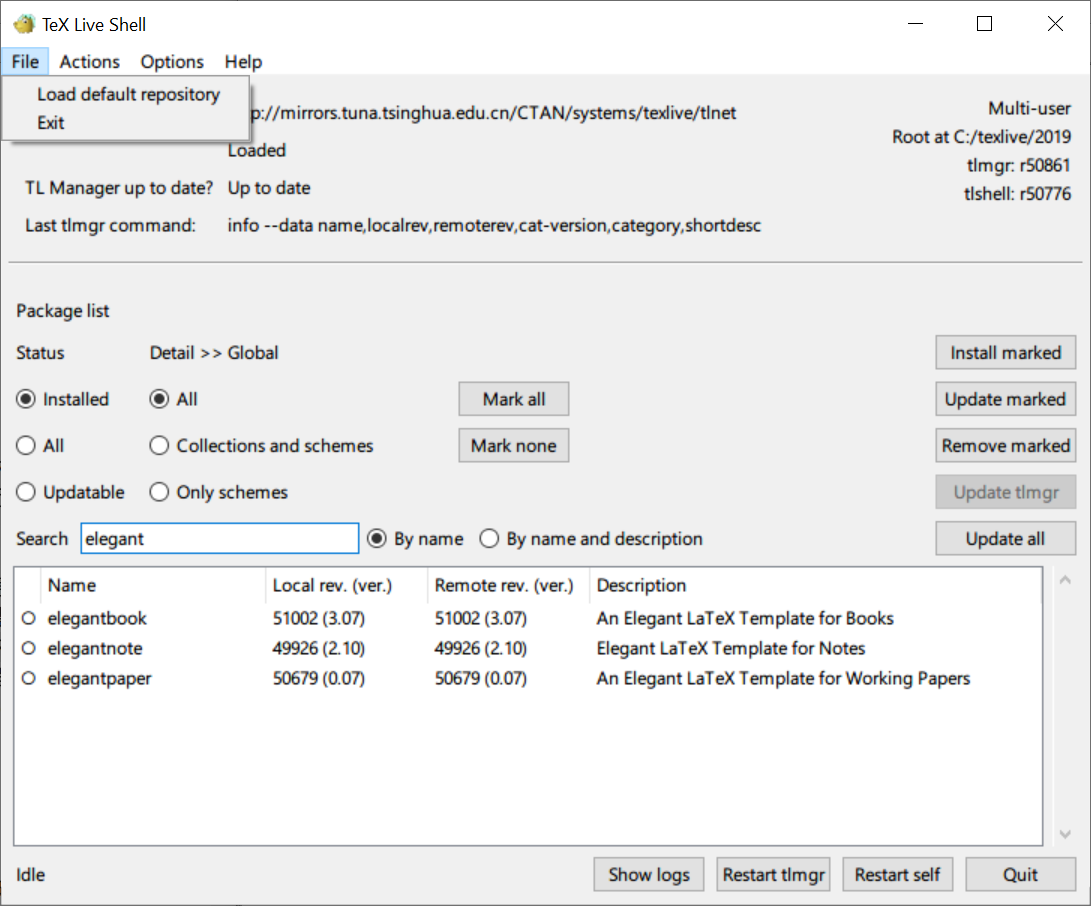
\includegraphics[width=0.7\textwidth]{tlshell.png}
\caption{使用 \TeX{} Live Shell 安装 ElegantBook 模板}
\end{figure}


\begin{table}[!htbp]
  \centering
  \caption{捐赠榜}
    \begin{tabular}{crcc}
    \toprule
    捐赠者   & 金额 & 时间 & 渠道 \\
    \midrule
    Lerh  & 10 元  & 2019/05/15 & 微信 \\
    越过地平线 & 10 元    & 2019/05/15 & 微信 \\
	大熊 &  20 元 & 2019/05/27 & 微信 \\
	佚名 & 10 元 & 2019/05/30 & 微信\\
	\href{http://www.latexstudio.net/}{latexstudio.net} & 666 元 & 2019/06/05 & 支付宝\\
	Cassis & 11 元 & 2019/06/30 & 微信\\
	佚名 & 10 元 & 2019/07/23 & 微信\\
    \bottomrule
    \end{tabular}%
\end{table}%